\chapter[Crossbow MIB5X0 Board]{Crossbow MIB5X0 Board}

\section{Introduction}

This chapter describes the support done in \ee\ for the Crossbow
MIB5X0 Board. Please note that both boards mib510 and mib520 are
supported, enabling the programming of the mica2 and micaz nodes (see
Figure \ref{fig:mib520}).

\begin{figure}
  \begin{center}
    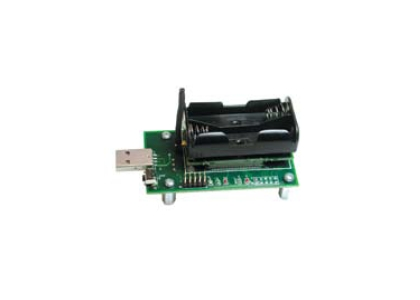
\includegraphics[width=6cm, bb=0 0 420 300]{images/mibmicaz.jpg}
  \end{center}
  \caption{Crossbow MIB520 Board and MicaZ.}
  \label{fig:mib520}
\end{figure}

The Mib520 is a low cost, efficient development board produced by
Crossbow with interfaces to JTAG and USB \cite{mibmicaz}.

To configure the usage of both MIB510 Board and MIB520 board, the user
has to specify an appropriate \const{BOARD_DATA}, as in the following example:

\begin{lstlisting}
  ...
  BOARD_DATA = XBOW_MIB5X0 {
    ...
  }
  ...
\end{lstlisting}

% -------------------------------------------------------------------

\section{LEDs}

The MIB5X0 Board has a set of 3 LEDs attached to the PORTA pins of the
microcontroller. To use the LEDs on the Board, the
developer should specify the \const{USELEDS} attribute as TRUE, as in
the following example:

\begin{lstlisting}
  ...
  BOARD_DATA = XBOW_MIB5X0 {
    USELEDS = TRUE;
    ...
  }
  ...
\end{lstlisting}

The following subsections will describe the functions available to
control the Crossbow MIB5X0 LEDs.


\begin{function_nopb2}{EE\_led\_1\_on}{EE_led_1_on:mib5x0}
  \synopsis{void EE_led_1_on(void);}
  
  \begin{fundescription}
    The function turns on LED 1.
  \end{fundescription}
  
%  \begin{funparameters}
%    \fpar{none}{None in this function.}
%  \end{funparameters}
  
%  \begin{funreturn}
%    \fret{void}{The function does not return a value.}
%  \end{funreturn}
  
%  \begin{funconformance}
%  \end{funconformance}
\end{function_nopb2}

\begin{function_nopb2}{EE\_led\_1\_off}{EE_led_1_off:mib5x0}
  \synopsis{void EE_led_1_off(void);}
  
  \begin{fundescription}
    The function turns off LED 1.
  \end{fundescription}
  
%  \begin{funparameters}
%    \fpar{none}{None in this function.}
%  \end{funparameters}
  
%  \begin{funreturn}
%    \fret{void}{The function does not return a value.}
%  \end{funreturn}
  
%  \begin{funconformance}
%  \end{funconformance}
\end{function_nopb2}

\begin{function_nopb2}{EE\_led\_2\_on}{EE_led_2_on:mib5x0}
  \synopsis{void EE_led_2_on(void);}
  
  \begin{fundescription}
    The function turns on LED 2.
  \end{fundescription}
  
%  \begin{funparameters}
%    \fpar{none}{None in this function.}
%  \end{funparameters}
  
%  \begin{funreturn}
%    \fret{void}{The function does not return a value.}
%  \end{funreturn}
  
%  \begin{funconformance}
%  \end{funconformance}
\end{function_nopb2}

\begin{function_nopb2}{EE\_led\_2\_off}{EE_led_2_off:mib5x0}
  \synopsis{void EE_led_2_off(void);}
  
  \begin{fundescription}
    The function turns off LED 2.
  \end{fundescription}
  
%  \begin{funparameters}
%    \fpar{none}{None in this function.}
%  \end{funparameters}
  
%  \begin{funreturn}
%    \fret{void}{The function does not return a value.}
%  \end{funreturn}
  
%  \begin{funconformance}
%  \end{funconformance}
\end{function_nopb2}

\begin{function_nopb2}{EE\_led\_3\_on}{EE_led_3_on:mib5x0}
  \synopsis{void EE_led_3_on(void);}
  
  \begin{fundescription}
    The function turns on LED 3.
  \end{fundescription}
  
%  \begin{funparameters}
%    \fpar{none}{None in this function.}
%  \end{funparameters}
  
%  \begin{funreturn}
%    \fret{void}{The function does not return a value.}
%  \end{funreturn}
  
%  \begin{funconformance}
%  \end{funconformance}
\end{function_nopb2}

\begin{function_nopb2}{EE\_led\_3\_off}{EE_led_3_off:mib5x0}
  \synopsis{void EE_led_3_off(void);}
  
  \begin{fundescription}
    The function turns off LED 3.
  \end{fundescription}
  
%  \begin{funparameters}
%    \fpar{none}{None in this function.}
%  \end{funparameters}
  
%  \begin{funreturn}
%    \fret{void}{The function does not return a value.}
%  \end{funreturn}
  
%  \begin{funconformance}
%  \end{funconformance}
\end{function_nopb2}


